\documentclass[a4paper, 12pt]{report}
\usepackage{geometry}
\geometry{a4paper,hmargin={3cm,2.5cm},vmargin={2.5cm,2.5cm}}

\usepackage{geometry}
\geometry{
    a4paper,
    headheight=15pt,
    hmargin={3cm,2.5cm},
    vmargin={2.5cm,2.5cm}
}
 
\usepackage{amsfonts} % if you want blackboard bold symbols e.g. for real numbers
\usepackage{multicol}
\usepackage{float}
\usepackage{blindtext}
\usepackage{fancyhdr}
\pagestyle{fancy}
\usepackage{hyperref}
\usepackage{amsmath} % for 'bmatrix' environment
\usepackage{tikz}
\usetikzlibrary{calc}
\usepackage{eso-pic}
\usepackage{lipsum}
\usepackage{longtable}
\setlength{\parindent}{0em}
\setlength{\parskip}{1em}
\usepackage{biblatex} %Imports biblatex package
\addbibresource{main.bib} %Import the bibliography file
\usepackage{scrextend}
\usepackage{subfig}
\usepackage{graphicx} % for jpeg or pdf pictures
\usepackage{lmodern}
\usepackage{minted}
\usepackage{colortbl}
\usepackage[section]{placeins}

\hypersetup{
    colorlinks=true,
    linkcolor=blue,
    filecolor=magenta,      
    urlcolor=cyan,
}

% acronyms
\usepackage{acronym} 

%\lhead{}
%\rhead{Project Report - Preferential Attachment with machine learning}
%\lfoot{Open University of Israel - Dept. of Mathematics and Computer Science}

%========================= BEGIN DOCUMENT ================================= %

\begin{document}

% The frontmatter environment for everything that comes with roman numbering
\newenvironment{frontmatter}{}{}
\begin{frontmatter}

%========================= TITLE-PAGE ================================= %
\begin{titlepage}

\begin{center}
\large\textbf{The Open University of Israel}\\
\textit{Department of Mathematics and Computer Science}

% LOGO (OU) -------------------------------------
\begin{center}
\begin{figure}[!ht]
\centering

\includegraphics[width=0.3\linewidth]{./logo}
\end{figure}
\end{center}
%------------------------------------------------

\textup{\large A PROJECT REPORT\\on}

\begin{LARGE}
{\textbf {Preferential Attachment\\using machine learning}}
\end{LARGE}

\textit{SUBMITTED BY}

\begin{large}\textbf{YOSSI COHEN}\\\textit{THE OPEN UNIVERSITY}\end{large}

\textit{UNDER THE GUIDANCE OF}

\begin{large}\textbf{PROF. YOSSI GIL}\\\textit{THE TECHNION}\end{large}

\begin{large}\textit{(2020-2021)}\end{large}

\end{center}
\end{titlepage}

%========================== ACKNOWLEDGEMENT ================================== %

\section*{\begin{center}\textit{ACKNOWLEDGEMENT}\end{center}}

\textit{I would like to thank \emph{Prof. Yossi Gil} for encouraging me to go ahead and for his continuous guidance with the project and assistance in preparing this report.}

\textit{I would also like to thank all those, who have directly or indirectly helped me for the completion of the work during this project.}

%========================= TABLE OF CONTENTS ================================= %
\tableofcontents
\listoffigures
\listoftables

%========================== ABSTRACT ================================== %

\begin{abstract}
Power laws appear widely in physics, biology, earth and planetary sciences, economics and finance, computer science, demography, and social sciences. For instance, the distributions of the sizes of cities, earthquakes, forest fires, solar flares, moon craters, and people’s personal fortunes all appear to follow power laws.

In his paper ``Power laws, Pareto distributions, and Zipf’s law", Newman reviews some of the empirical evidence for the existence of power-law forms and the theories proposed to explain them.

In this project, we show that a key property of such \textit{power law} distribution, concretely  \textit{Yule-Simon distribution}, can be in fact estimated with a reasonable accuracy using machine learning methods.

\vspace{0.3cm}

\textbf{Keywords}: \it{Preferential Attachment, Machine Learning}
\end{abstract}
%================================================ %
% The frontmatter environment for everything that comes with roman numbering %
\end{frontmatter}
%%%%%%%%%%%%%%%%%%%%%%%%%%%%%%%%%%%%%%%%%%%%%%%%%%%%%%%%%%%%%%%%%%%%%%%%%%%%%%%%%%%%%%%%%%%%%%%%


\pagenumbering{arabic}
%%%%%%%%%%%%%%%%%%%%%%%%%%%%%%%%%%%% MAIN TEXT STARTS HERE %%%%%%%%%%%%%%%%%%%%%%%%%%%%%%%%%%%%%
\chapter{INTRODUCTION}

\section{Background}
In his paper ``Power laws, Pareto distributions, and Zipf’s law" \cite{newman}, Newman reviews some of the empirical evidence for the existence of power-law forms and the theories proposed to explain them. This section is mostly a short summary of this paper.

Many of the things that we measure have a \textit{typical value} around which individual measurements are centred. A simple example would be the heights of human beings. Most adult human beings (in the U.S) are about 180 cm tall. There is some variation around this figure, notably depending on sex, but we never see people who are 10 cm tall, or 500 cm. Other examples would be e.g., shoe size and speed of cars on the motorway.

\begin{figure}[!ht]
\centering
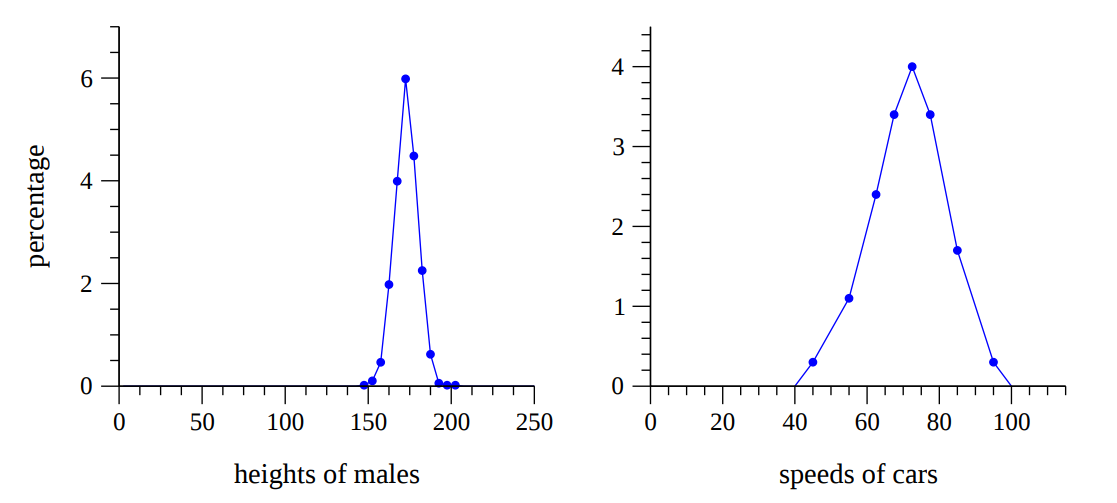
\includegraphics[width=0.7\linewidth]{./heights-of-males}
\caption{
    Distributions centered around a typical value.  
    Left: histogram of heights in centimetres of American males. Data from the National Health Examination Survey,
    1959 – 1962 (US Department of Health and Human Services). Right: histogram of speeds in miles per hour of cars on UK
    motorways. Data from Transport Statistics 2003 (UK Department for Transport).
}

\label{fig:heights-of-males}
\end{figure}

However, not all things we measure are peaked around a typical value. Some vary over an enormous dynamic range, sometimes many orders of magnitude. 

When the probability of measuring a particular value of some quantity varies inversely as
a power of that value, the quantity is said to follow a \textit{power law}, also known as \textit{Zipf’s law} or the \textit{Pareto distribution}. 


Power laws appear widely in physics, biology, earth and planetary sciences, economics and finance, computer science, demography, and social sciences. For instance, the distributions of the sizes of cities, earthquakes, forest fires, solar flares, moon craters, and people’s personal fortunes all appear to follow power laws.

\begin{figure}[!ht]
\centering
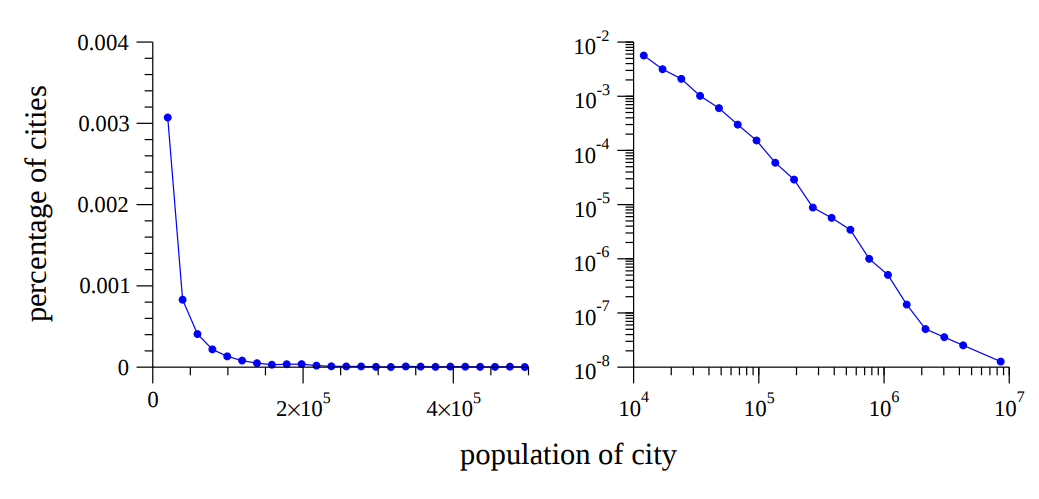
\includegraphics[width=0.7\linewidth]{./population-of-cities}
\caption{
Population of cities.  
Left: histogram of the populations of all US cities with population of 10000 or more. Right: another histogram of
the same data, but plotted on logarithmic scales. The approximate straight-line form of the histogram in the right panel
implies that the distribution follows a power law. Data from the 2000 US Census.
}
\label{fig:populations-of-cities}
\end{figure}

Figure \ref{fig:populations-of-cities} (left) shows the histogram of city sizes. In the same figure (right), the histogram is shown in a log-log scale. The histogram, plotted in this fashion follows quite closely a straight line (this observation is attributed to Zipf).

Let $p(x)dx$ be the fraction of cities with population between $x$ and $x+dx$. If the histogram is a straight line on log-log scales, then $ln p(x) = - \alpha ln(x) + c$, where $\alpha$ and $c$ are constants. Taking
the exponential of both sides, we get:

\begin{equation}
\label{eq:powerlaw}
p(x) = Cx^{- \alpha}
\end{equation}
with $C = e^c$.

Distributions of the form \ref{eq:powerlaw} are said to follow a power law. The constant $\alpha$ is called the exponent of the power law. (The constant $C$ is mostly uninteresting; once $\alpha$ is fixed, it is determined by the requirement that the distribution $p(x)$ sum to 1).


\subsection{Measuring power laws}
The standard strategy for identifying power-law behaviour is to plot a histogram on a logarithmic scale where it appears as a straight line. Figure \ref{fig:histogram-1-million} shows a fake data set generated from 1 million random numbers with a power law distribution $p(x) = Cx^{- \alpha}$ with $\alpha=-2.5$

Panel (a) of the figure shows a normal histogram of the numbers, produced by binning them into bins of equal size $(0.1)$.

Plotting the histogram on logarithmic scales reveals the straight line behavior as can be seen in Panel (b). However, the right-hand end of the distribution is noisy because of sampling errors. In this region, each bin only has a few samples in it, if any. Therefore the fractional fluctuations in the bin counts are large and this appears as a noisy curve on the plot.

In panel (c), the width of the bins in the histogram is plotted with \textit{logarithmic binning}, meaning the width of each bin is a multiple of the previous one $(0.1,0.2,0.4,...)$. The sample count is then normalized by dividing the number of samples in a bin of width $\Delta x$ by $\Delta x$. This means the bins in the tail of the distribution get more samples than they would if the bin sizes were fixed, and this reduces the statistical errors in the tail.

\begin{figure}[!ht]
\centering
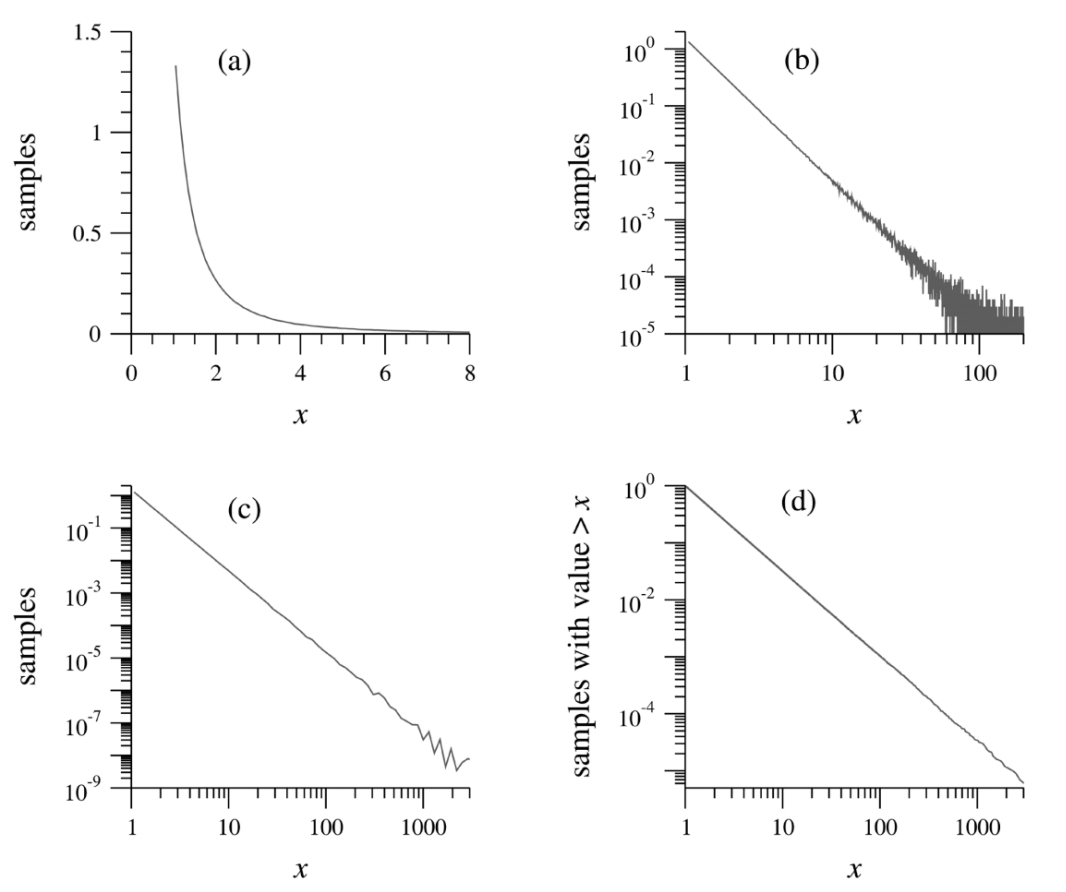
\includegraphics[width=0.7\linewidth]{./histogram-1-million}
\caption{
    (a) Histogram of the set of 1 million random numbers described in the text, which have a power-law distribution with exponent a = 2.5. (b) The same histogram on logarithmic scales. Notice how noisy the results get in the tail towards the right-hand side of the panel. This happens because the number of samples in the bins becomes small and statistical fluctuations are therefore large as a fraction of sample number. (c) A histogram constructed using ‘logarithmic binning’. (d) A cumulative histogram or rank/frequency plot of the same data. The cumulative distribution also follows a power law, but with an exponent of a – 1 = 1.5
}
\label{fig:histogram-1-million}
\end{figure}

Even with logarithmic binning there is still some noise in the tail, although it is sharply decreased. As long as $\alpha > 1$, the number of samples per bin goes down as $k$ increases and the bins in the tail will have more statistical noise than those that precede them. Most power-law distributions occurring in nature have $2 \leq \alpha \leq 3$ \cite{newman}, so noisy tails are the norm.

Another method of plotting the data shown in panel (d) is to calculate a \textit{cumulative distribution function}, in which we make a plot of the probability $P(x)$ that $x$ has a value greater than or equal to $x$:

\begin{equation}
\label{eq:cumsum}
p(x) = \int_{x}^{\infty} p(x')\, dx'
\end{equation}

The \textit{cumulative distribution} also follows power law, but with an exponent of $\alpha-1 = 1.5$. Thus, we get again a straight line but with a shallower slope.

\section{Motivation}
We know the value of the exponent $\alpha$ for the artificial data set since it was generated deliberately to have a particular value, but in practical situations we would often like to \textbf{estimate $\alpha$ from observed data}.

It is known \cite{newman} that one way of doing this would be to fit the slope of the line in plots like figures \ref{fig:histogram-1-million} (b), (c) or (d), and this is the most commonly used method.
Unfortunately, it is known to introduce systematic biases into the value of the exponent [20], so it should not be relied upon. For example, a least-squares fit of a straight line to
figure 3 (b) gives a = 2.26 +0.02, which is clearly incompatible with the known value of a= 2.5 from which the data were generated.

\textbf{In this project}, we develop an alternative and reliable method for extracting the exponent with an acceptable error using \textit{Deep Learning} methods. Then, this preliminary result will motivate further research on harnessing such methods for identifying power law distributions and maybe classifying distributions as such.

\section{Preferential Attachment}
\textit{Preferential Attachment} is a another model which has properties of the \textit{power law} distribution. It is best explaining the \textit{Preferential Attachment} model by example (e.g: on a node network).
\begin{enumerate}
\small
    \item We start with two nodes connected by an edge.
    \item At each time step, add a new node with an edge connecting it to a single existing node. 
    \item Choose the node to connect to at random with probability proportional to the node`s current degree.
    \item The probability of connecting to a node $u$ of degree $k_u$ is $\frac{k_u}{\sum_j{k_j}}$
\end{enumerate}

\section{Yule process}
\textit{Preferential Attachment} may be realized using the \textit{Yule process}  \cite{yule-simon-distribution}.

An example \textit{Yule process} is implemented by the following procedure:

Distribute $N \gg 1$ balls among urns iteratively using \textit{preferential attachment} policy.

At each step, add a urn with initial $k_0$ balls and distribute $m$ balls among urns with a probability proportional to the number of balls in each urn.

Run as many iterations as necessary to distribute all $N$ balls.

Parameters:
\small
\begin{addmargin}[1cm]{1cm}% 1cm left, 1cm right
    $N: N \gg 1$, the total number of balls we wish to distribute.
    
    $m: 1 \leq m \leq 10$, the number of balls distributed at each iteration.
    
    $k_0: 1 \leq k_0 \leq 10$, the initial number of balls for a newly created urn.
\end{addmargin}

{\fontfamily{qcr}\selectfont
As an example: N = 10000; k0 = 10; m = 3
}

\begin{figure}[!ht]
\centering
    % Requires \usepackage{graphicx}
    \subfloat[]{
        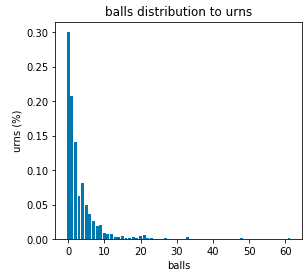
\includegraphics[width=0.25\textwidth]{yule-histogram}
        \label{fig:yule-process-histograms-1a}
    }
    \hspace{0.5cm}
    \subfloat[]{
        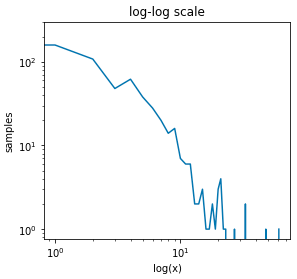
\includegraphics[width=.25\textwidth]{yule-log}
        \label{fig:yule-process-histograms-1b}
    }
    \hspace{0.5cm}
    \subfloat[]{
        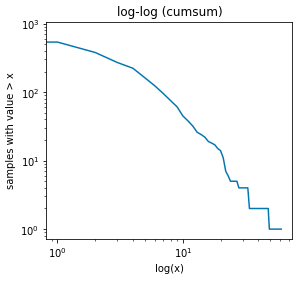
\includegraphics[width=.25\textwidth]{yule-log-cumsum}
        \label{fig:yule-process-histograms-1c}
    }
    \label{fig:yule-process-histograms}
    \caption[]{
        Yule process histograms: 
        $(a)$ A histogram of $N=10,000$ balls distributed to urns with \textit{Yule distribution}.
        $(b)$ The same histogram on logarithmic scale.
        $(c)$ A cumulative histogram of the same data.
    }
\end{figure}

\chapter{PROJECT IMPLEMENTATION}

\section{Problem Statement}
Given a collection of generated samples drawn from the \textit{Yule-Simon} distribution with a known exponents $\alpha_1,...,\alpha_n$, the \textbf{task} of the learning model is to \textbf{predict $\alpha$} for a single sample of length $\geq m$ within a specified bounded error:
$$\mid prediced(\alpha) - \alpha \mid \; \leq \; 0.01$$

A simulator will be written to generate data for learning and testing purposes, so there is no limit on the available dataset size.

\section{Dataset}
\label{dataset}

The datasets used in the project were generated using the \textbf{\textit{yulesimon}} distribution from \textbf{\textit{scipy.stat}} package.

As an example, the following will generate $1,000$ random numbers for a given $alpha=\alpha$
\begin{equation}
\label{eq:yulesimon.rvs}
r = yulesimon.rvs(alpha=\alpha, size=1,000)
\end{equation}
$generate\_data()$ function uses \ref{eq:yulesimon.rvs} to draw $N$ random samples for each $\alpha$ in the range: $[min\_alpha, max\_alpha]$ with $S$ $yulesimon.rvs$ calls for each $\alpha$, yielding the following dataset:
(concatenated as a single matrix $YS = [(M * S), N]$)

\begin{itemize}
\small
  \item $N$ (columns): number of samples drawn for a given $\alpha$
  \item $M$: number of different $\alpha$ generated in the range: [$min\_\alpha$, $max\_\alpha$]
  \item $S$: number of samples per $\alpha$ (number of calls to $yulesimon.rvs$ with same $\alpha$)
\end{itemize}
\[
samples(\alpha_1) = \begin{bmatrix} 
    r^{(\alpha_1)}_{1,1} & r^{(\alpha_1)}_{1,2} & \dots & r^{(\alpha_1)}_{1,N} & \\
    r^{(\alpha_1)}_{2,1} & r^{(\alpha_1)}_{2,2} & \dots & r^{(\alpha_1)}_{2,N} & \\
    \vdots & \ddots & \vdots & \\
    r^{(\alpha_1)}_{S,1} & r^{(\alpha_1)}_{S,2} & \dots & r^{(\alpha_1)}_{S,N} & \\
\end{bmatrix}
\]

\[
samples(\alpha_2) = \begin{bmatrix} 
    r^{(\alpha_2)}_{1,1} & r^{(\alpha_2)}_{1,2} & \dots & r^{(\alpha_2)}_{1,N} & \\
    r^{(\alpha_2)}_{2,1} & r^{(\alpha_2)}_{2,2} & \dots & r^{(\alpha_2)}_{2,N} & \\
    \vdots & \ddots & \vdots & \\
    r^{(\alpha_2)}_{S,1} & r^{(\alpha_2)}_{S,2} & \dots & r^{(\alpha_2)}_{S,N} & \\
\end{bmatrix}
\]
\[
\vdots
\]
\[
samples(\alpha_M) = \begin{bmatrix} 
    r^{(\alpha_M)}_{1,1} & r^{(\alpha_M)}_{1,2} & \dots & r^{(\alpha_M)}_{1,N} & \\
    r^{(\alpha_M)}_{2,1} & r^{(\alpha_M)}_{2,2} & \dots & r^{(\alpha_M)}_{2,N} & \\
    \vdots & \ddots & \vdots & \\
    r^{(\alpha_M)}_{S,1} & r^{(\alpha_M)}_{S,2} & \dots & r^{(\alpha_M)}_{S,N} & \\
\end{bmatrix}
\]

A histogram $H$ is then created for rows of $[YS]$ where: 
\begin{equation}
\label{eq:nbins}
\textbf {nbins} = max(YS)
\end{equation}
$H$ is therefore a matrix of size $[(M * S), nbins]$.  Each row $H_i$ is a histogram with $nbins$ corresponding to an input row $YS_i$. $H_i$ is counting the number of samples of the corresponding input row $YS_i$ in each bin.

Finally, we apply $\log$ on $H$ rows to get the input $X$ to the learning process:
\begin{equation}
\label{eq:log_H}
    {\textbf X} = \log(H)
\end{equation}
We set the output $y$ as:
\begin{equation}
\label{eq:y}
{\textbf y} = \begin{bmatrix} 
    \alpha_1 & \\
    \alpha_1 & \\
    \hdots & \\
    \alpha_2 & \\
    \alpha_2 & \\
    \hdots & \\
    \alpha_M & \\
\end{bmatrix}
\end{equation}

\begin{itemize}
  \item NOTE: $y$ contains $S$ copies for each $\alpha_1...\alpha_M$ for total length of $[S*M]$
\end{itemize}

$generate\_data()$ function returns: $(X, y, nbins)$ as an input for the learning process.

An example of a single row in $X = \log(H)$ is shown in figure  \ref{fig:yule-simon-log-scale}

\begin{figure}[!ht]
\centering
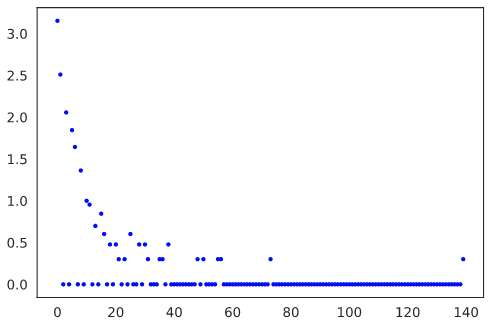
\includegraphics[width=0.7\linewidth]{./dataset}
\caption{Yule-Simon distribution in log-scale $X = \log(H)$ for $\alpha\in[2.0,3.0], N=2,048$ (140 bins = $max(X)$)}
\label{fig:yule-simon-log-scale}
\end{figure}

\textit{Note}: We will see later that padding bins with zero value at the right end improves the $NN$ model accuracy (figure  \ref{fig:yule-simon-log-scale-zeros-padding})

\begin{figure}[!ht]
\centering
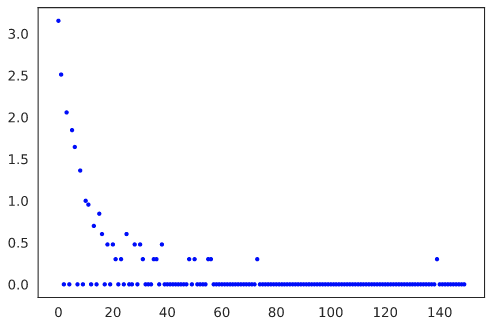
\includegraphics[width=0.7\linewidth]{./dataset-zeros}
\caption{Yule-Simon distribution in log-scale with right zero padding}
\label{fig:yule-simon-log-scale-zeros-padding}
\end{figure}

\section{DNN}
In practical situations we would often like to estimate $\alpha$ from observed data \cite{newman}. One way to do this would be to fit the slope of the line in plots like figures (\ref{fig:yule-process-histograms-1b}), (\ref{fig:yule-process-histograms-1c}) Unfortunately, it is known to introduce systematic biases into the value of the exponent $\alpha$, so it should not be relied
upon.

\textit{DNN (Deep Neural Network)}, not like simple line-fit models, can learn complex patterns. Thus, the first approach used in this project was a \textit{Regression DNN}.

\subsection{Experiments}
In order to streamline the experiments, a $trial()$ helper function has been defined.

$trial()$ runs several iterations as defined by the following arguments:

\begin{itemize}
  \item $N\_range$: a set $\{I\}$ where $\{N = 2^{i\in I}\}$ are the number of samples to draw from \textit{yulesimon} distribution for a given $\alpha$.
  \item $hstack\_zeros$: whether to right append zeros to the generated \textit{dataset}.
  \item $\{random\_states\}$: a set of random state values to run the trained model in each iteration.
\end{itemize}

The $trial()$ function calls $generate\_data(N)$ to produce growing size datasets. For each \textit{dataset} generated, $trial()$ creates a corresponding \textit{DNN} model. It then iterates over the given $\{random\_states\}$ set to train and test the model.

$trial()$ function returns:
\begin{itemize}
\small
  \item $[N]$: the list of $N's$ used in each iteration.
  \item $[sqrt\_mse]$: the corresponding $\sqrt{MSE(\alpha)}$ for each iteration.
  \begin{itemize}
    \item $sqrt\_mse = sqrt(mean\_squared\_error(\alpha\_test, \alpha\_pred))$
  \end{itemize}
  \item $[avg\_abs\_errors]$: AVG of absolute error for each iteration.
  \begin{itemize}
    \item $avg\_abs\_errors = avg(abs(\alpha\_test - \alpha\_pred))$
  \end{itemize}
  \item $[std\_abs\_errors]$: \textsc{std} of the absolute error for each iteration.
  \begin{itemize}
    \item $std\_abs\_errors = std(avg\_abs\_errors)$
  \end{itemize}
\end{itemize}

\subsection{DNN}

\subsubsection{Purpose of experiment}
Check the precision of evaluating $\alpha$ using \textit{DNN}

\subsubsection{Course of experiment}
The \textit{DNN} model was implemented using \textit{Keras} under \textit{Jupyter Notebook}.

The neural network has an input layer which is fed with the dataset described in section \ref{dataset}. It has couple of fully connected hidden layers with \textit{relu} activation and an output layer with a \textit{linear} activation. All layers use batch normalization, \textit{Adam} optimizer, kernel and activation \textit{regularization}. The loss function used is \textit{\ac{MSE}}.

\subsubsection{Summary of DNN hyper parameters}
xxx

I have made little attempt to optimize the parameters of the network, and
so improved performance may be obtained by exploring other values.

Input to the network has been splitted to \textit{TRAIN}, \textit{VALIDATION} and \textit{TEST} sets.

Model training used \textit{early stopping} and \textit{reduce learning-rate on plateau}.

Training used \textit{batch size} of $32$ and couple of hundred \textit{epochs}.

\textit{Learning Curves} (train/validation) have been used to identify and eliminate \textit{overfitting}.

\textit{NOTE}: for each $N$, we run several train/test cycles, each with different random state and average results:
\begin{minted}{python}
for rs in random_states:
    model = train(model, X_train, y_train, ..., random_state=rs)
    y_pred = model.predict(X_test)
    sqrt_mse = sqrt(MSE(y_test, y_pred))
    avg_sqrt_mse += sqrt_mse
    ...
avg_sqrt_mse \= len(random_states)
\end{minted}

\subsubsection{Results}
Running \textit{DNN} on $100$ alpha values with 100 samples per alpha yield the following:

\begin{table}[h!]
    \centering
    \begin{tabular}{r r r} 
        $N$ & input-shape & $E\left(\sqrt{MSE(\alpha)}\;\right)$ \\
        \hline
        32 & (10000, 34) & 0.04326 \\ 
        64 & (10000, 20) & 0.01430 \\
        128 & (10000, 46) & 0.01480 \\
        \rowcolor{yellow}
        256 & (10000, 21) & 0.01041 \\
        512 & (10000, 33) & 0.00908 \\ 
        1,024 & (10000, 63) & 0.00985 \\ 
        2,048 & (10000, 140) & 0.01002 \\ 
    \end{tabular}
    \caption{$E\left(\sqrt{MSE(\alpha)}\right)$ for \textit{DNN}}
    \label{table:dnn-sqrt-mse}
\end{table}

\subsubsection{Conclusions}
\textit{DNN} is shown to achieve a stable error rate around $0.01$ for $N \geq 256$. This results are better than those reported so far $(\pm 0.02)$ for larger datasets using mathematical methods \cite{newman}. 

\subsection{DNN with zero padding}

\subsubsection{Purpose of experiment}
Check the precision of evaluating $\alpha$ using \textit{DNN} with right zeros padding.

\subsubsection{Course of experiment}
Using the same \textit{DNN} as before, We've used the same input as above with right zeros padding.
The purpose of padding the zeros to the right was to ease the network learning process.

\subsubsection{Results}
Running \textit{DNN} on the same input as above with right padding zeros yield the following:
\begin{table}[h!]
    \centering
    \begin{tabular}{r r r} 
        $N$ & input-shape & $E\left(\sqrt{MSE(\alpha)}\;\right)$ \\
        \hline
        32 & (10000, 44) & 0.04341 \\ 
        64 & (10000, 30) & 0.01435 \\
        128 & (10000, 56) & 0.01506 \\
        256 & (10000, 31) & 0.01066 \\
        \rowcolor{yellow}
        512 & (10000, 43) & \textbf{0.00798} \\ 
        1,024 & (10000, 73) & 0.01143 \\ 
        \rowcolor{yellow}
        2,048 & (10000, 150) & \textbf{0.00789} \\ 
    \end{tabular}
    \caption{$E\left(\sqrt{MSE(\alpha)}\right)$ for \textit{DNN} with zero padding}
    \label{table:dnn-zero-sqrt-mse}
\end{table}

\subsubsection{Conclusions}
Comparing the results in table \ref{table:dnn-zero-sqrt-mse} to those in table \ref{table:dnn-sqrt-mse}, it can be seen that padding with zeros improved somewhat but not much. 

\subsection{DNN additional experiments}
Before moving to describe the \textit{CNN} based model, it should be mentioned that several additional experiments were taken based on the \textit{DNN} model. Two of them are described here.

Trying to help the \textit{DNN} model to capture the shape of the input, a \textit{sliding-avg} and a \textit{sliding-sum} manipulations on the input have been taken.

\subsubsection{DNN sliding-avg}
For example, suppose a row of the input is:
\begin{minted}{python}
    [1 2 3 4 5 6 7]
\end{minted}

The \textit{sliding-avg} works row-wise on window sizes of $2^i$ where $i \in \{1,2,...\}$.

In the example above, the valid window sizes are:
\begin{minted}{python}
    window_sizes: [2, 4]
\end{minted}

The \textit{sliding-avg} copy a row of the input as is ($1..7$). Then, start by sliding a window of size 2 (stride=1) and appends the avg. of every two elements ($avg(1,2)$, $avg(2,3)$, ...). Then it begins from the start with a sliding window of size 4 (stride=1) averaging every 4 elements. Output follows:
\begin{minted}{python}
    [1.  2.  3.  4.  5.  6.  7.  1.5 2.5 3.5 4.5 5.5 6.5 2.5 3.5 4.5 5.5]
\end{minted}

\subsubsection{DNN sliding-sum}
The \textit{sliding-sum} goes the same way as the \textit{sliding-avg} but appends the sum elements of $window\_size=2$, then $window\_size=4$, etc. Output follows:
\begin{minted}{python}
    [1.  2.  3.  4.  5.  6.  7.  3 5 7 9 11 13 10 14 18 22]
\end{minted}

\subsubsection{Sliding-windows results}
It appeared that the sliding method didn't improve performance.

\section{CNN}
Although \textit{DNN} yields relatively acceptable errors ($\approx 0.01$ for $N \geq 256$), a $~CNN$ model (\textit{Conv1D}) has been investigated.

A \textit{Conv1D} layer creates a convolution kernel (filter) that is convolved with its input over a single spatial (or temporal) dimension to produce a tensor of outputs.

Filters learn feature representations of the input. The more representations used, the better the performance will be (generally not always, having more filters than needed can also lead to overfitting).

\subsubsection{Purpose of experiment}
Check the precision of evaluating $\alpha$ using \textit{CNN} (Conv1D).

\subsubsection{Course of experiment}
In the first experiment, we used \textit{Conv1D} with 32-filters of size 3 and a $relu$ activation, followed by max-pooling $(pool\_size=2)$ and two $Dense$ layers $Dense(64, relu)$ and $Dense(1)$. The loss is again $MSE$ and the optimizer used was \textit{Adam}.

The model is fairly simple:
\begin{minted}{python}
def create_cnn_model(n_features, filters=32):
    model = Sequential()
    model.add(Conv1D(32, 3, activation='relu', input_shape=(n_features, 1)))
    model.add(MaxPooling1D(pool_size=2))
    model.add(Flatten())
    model.add(Dense(64, activation='relu'))
    model.add(Dense(1))
    model.compile(loss='mse', optimizer='adam')
    return model
\end{minted}

The \textit{CNN} model was tested the same way as the \textit{DNN} model using $trials()$ helper over the same inputs.

\subsubsection{Results}
Using \textit{CNN} as described above yield the following results:

\begin{table}[h!]
    \centering
    \begin{tabular}{r r r} 
        $N$ & input-shape & $E\left(\sqrt{MSE(\alpha)}\;\right)$ \\
        \hline
        32 & (10000, 34) & 0.04104 \\ 
        \rowcolor{yellow}
        64 & (10000, 20) & 0.01080 \\
        128 & (10000, 46) & 0.01146 \\
        256 & (10000, 21) & 0.00498 \\
        512 & (10000, 33) & 0.00365 \\ 
        1,024 & (10000, 63) & 0.00219 \\ 
        \rowcolor{yellow}
        2,048 & (10000, 140) & 0.00122 \\ 
    \end{tabular}
    \caption{$E\left(\sqrt{MSE(\alpha)}\right)$ for \textit{CNN}}
    \label{table:cnn-sqrt-mse}
\end{table}

\subsubsection{Conclusions}
Comparing the results in table \ref{table:cnn-sqrt-mse} to those in table \ref{table:dnn-sqrt-mse}, it can be seen that the error improved significantly, achieving an error expectation of $\pm 0.01$ even at $N \geq 64$ and improving down to $\pm 0.001$ (an order of magnitude) for $N \geq 2,048$.

This is far better than the results known so far \cite{newman}.

\subsection{CNN with zero padding}
\subsubsection{Purpose of experiment}
Check the precision of evaluating $\alpha$ using \textit{CNN} with right zeros padding.

\subsubsection{Course of experiment}
Running the same \textit{CNN} as described above with the same input and right zeros padding.

\subsubsection{Results}
This experiment yield the following results:
\begin{table}[h!]
    \centering
    \begin{tabular}{r r r} 
        $N$ & input-shape & $E\left(\sqrt{MSE(\alpha)}\;\right)$ \\
        \hline
        32 & (10000, 44) & 0.04111 \\ 
        64 & (10000, 30) & 0.01085 \\
        128 & (10000, 56) & 0.01161 \\
        256 & (10000, 31) & 0.00483 \\
        512 & (10000, 43) & 0.00329 \\ 
        1,024 & (10000, 73) & 0.00229 \\ 
        2,048 & (10000, 150) & 0.00110 \\ 
    \end{tabular}
    \caption{$E\left(\sqrt{MSE(\alpha)}\right)$ for \textit{CNN} with zero padding}
    \label{table:cnn-zeros-sqrt-mse}
\end{table}

\subsubsection{Conclusions}
Comparing the results in table \ref{table:cnn-sqrt-mse} to those in table \ref{table:cnn-zeros-sqrt-mse}, it can be seen that padding with zeros did not improve the error. 

\section{CNN multi-layer}
The second \textit{CNN} experiment used a multi-layer with multiple \textit{Conv1D} and \textit{pooling}.

\subsubsection{Purpose of experiment}
Check the precision of evaluating $\alpha$ using \textit{multi-layer CNN}.

\subsubsection{Course of experiment}
The multi-layer \textit{CNN} model is defined as follow:

\begin{minted}{python}
def create_cnn_model_multi_layer(n_features, filters=32):
    model = Sequential()
    # conv layer 1
    model.add(Conv1D(filters,
                     kernel_size=7, strides=1, 
                     activation='relu', 
                     input_shape=(n_features, 1)))
    # conv layer 2
    input_size = ( input_size + 2 * padding - kernel_size ) / strides  + 1
    model.add(Conv1D(filters, kernel_size=5, ...) 
    # pooling layer 1
    model.add(MaxPooling1D(pool_size=2))
    # conv layer 3
    model.add(Conv1D(filters, kernel_size=3, ...) 
    # pooling layer 2
    model.add(MaxPooling1D(pool_size=2))
    # flatten
    model.add(Flatten())
    # dense layer 1
    model.add(Dense(64, activation='relu'))
    # output layer
    model.add(Dense(1))
    model.compile(loss='mse', optimizer='adam', metrics=['mse'])
    return model
\end{minted}

\subsubsection{Results}
Running \textit{CNN multi-layer} on the same input as above yields the following:
\begin{table}[h!]
    \centering
    \begin{tabular}{r r r} 
        $N$ & input-shape & $E\left(\sqrt{MSE(\alpha)}\;\right)$ \\
        \hline
        32 & (10000, 44) & 0.04095 \\ 
        64 & (10000, 30) & 0.01097 \\
        128 & (10000, 56) & 0.01028 \\
        256 & (10000, 31) & 0.00474 \\
        512 & (10000, 43) & 0.00302 \\ 
        \rowcolor{yellow}
        1,024 & (10000, 73) & 0.00158 \\ 
        2,048 & (10000, 150) & 0.00096 \\ 
    \end{tabular}
    \caption{$E\left(\sqrt{MSE(\alpha)}\right)$ for \textit{CNN} multi-layer}
    \label{table:cnn-multi-sqrt-mse}
\end{table}

\subsubsection{Conclusions}
Comparing the results in table \ref{table:cnn-multi-sqrt-mse} to those in table \ref{table:cnn-sqrt-mse}, it can be seen that the error did not improve significantly relative to \textit{CNN}, achieving an error expectation of $\pm 0.001$ at $N \geq 1,024$ (an order of magnitude relative to \textit{DNN}).

\subsection{CNN multilayer with zero padding}
This experiment follows the previous ones using right zeros padding.

\subsubsection{Purpose of experiment}
Check the precision of evaluating $\alpha$ using \textit{multilayer CNN} with right zeros padding.

\subsubsection{Course of experiment}
As before, using the same network (\textit{CNN multilayer}) with the same input padded with zeros on the right. 

\subsubsection{Results}
This experiment yield the following results:
\begin{table}[h!]
    \centering
    \begin{tabular}{r r r} 
        $N$ & input-shape & $E\left(\sqrt{MSE(\alpha)}\;\right)$ \\
        \hline
        32 & (10000, 44) & 0.04150 \\ 
        64 & (10000, 30) & 0.01094 \\
        128 & (10000, 56) & 0.01075 \\
        256 & (10000, 31) & 0.00438 \\
        512 & (10000, 43) & 0.00274 \\ 
        1,024 & (10000, 73) & 0.00159 \\ 
        2,048 & (10000, 150) & 0.00068 \\ 
    \end{tabular}
    \caption{$E\left(\sqrt{MSE(\alpha)}\right)$ for \textit{CNN} multi-layer with zero padding}
    \label{table:cnn-multi-zeros-sqrt-mse}
\end{table}

\subsubsection{Conclusions}
As in the case of \textit{DNN}, padding with zeros did not improve the error significantly.

\section{METHODS COMPARISON}
Table \ref{table:sqrt-mse-comparison} summarise $\sqrt{MSE(\alpha)}$ for $N=2^i~ i\in\{5...11\}$ for the different methods used.
\begin{table}[!htb]
    \sffamily
    \scriptsize
    \caption*{
        $z$: right zero padding\\
        $m$: multi-layer CNN
    }
    \centering
    \begin{tabular}{r r r r r r r} 
        $N$ & $DNN$ & $DNN_z$ & $CNN$ & $CNN_z$ & $CNN_m$ & $CNN_{m,z}$ \\
        \hline
        32 & 0.043260 & 0.043405 & 0.041040 & 0.041108 & 0.040951 & 0.041504 \\ 
        64 & 0.014299 & 0.014351 & 0.010801 & 0.010851 & 0.010968 & 0.010939 \\
        128 & 0.014803 & 0.015061 & 0.011461 & 0.011613 & 0.010276 & 0.010751 \\
        256 & 0.010409 & 0.010662 & 0.004984 & 0.004832 & 0.004736 & 0.004380 \\
        512 & 0.009084 & 0.007984 & 0.003653 & 0.003293 & 0.003019 & 0.002745 \\
        1,024 & 0.009846 & 0.011425 & 0.002195 & 0.002291 & 0.001577 & 0.001586 \\
        2,048 & 0.010022 & 0.007886 & 0.001215 & 0.001096 & 0.000956 & 0.000675 \\
    \end{tabular}
    \caption{$\sqrt{MSE(\alpha)}$ comparison}
    \label{table:sqrt-mse-comparison}
\end{table}

Figure \ref{fig:mse-alpha-comparison} displays a (\textit{logarithmic}) plot of the errors for different $N's$ for each of the methods. The performance of the \textit{CNN} methods over the \textit{DNN} stands out.
\begin{figure}[!ht]
\centering
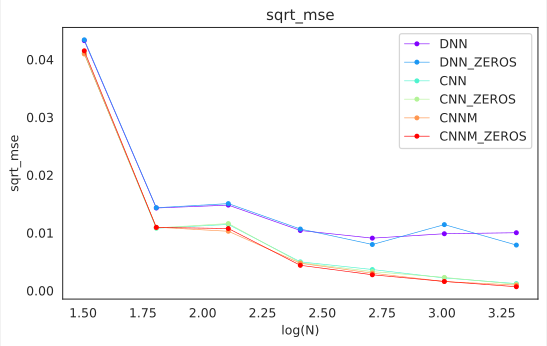
\includegraphics[width=0.7\linewidth]{./sqrt_mse_compare}
\caption{$MSE(\alpha)$ comparison}
\label{fig:mse-alpha-comparison}
\end{figure}

Table \ref{table:STD-comparison} summarise $STD$ of the different methods used.
This is another view showing the advantage of the \textit{CNN} based models.  
\begin{table}[!htb]
    \sffamily
    \scriptsize
    \centering
    \begin{tabular}{r r r r r r r} 
        $N$ & $DNN$ & $DNN_z$ & $CNN$ & $CNN_z$ & $CNN_m$ & $CNN_{m,z}$ \\
        \hline
    	32 & 0.023159 & 0.023944 & 0.025286 & 0.025220 & 0.025482 & 0.024870 \\
    	64 & 0.006112 & 0.005835 & 0.007213 & 0.007136 & 0.007140 & 0.007112 \\
    	128 & 0.007661 & 0.007169 & 0.007652 & 0.007497 & 0.006669 & 0.006585 \\
    	256 & 0.003591 & 0.002905 & 0.003501 & 0.003425 & 0.002951 & 0.003059 \\
    	512 & 0.002553 & 0.002169 & 0.002071 & 0.002125 & 0.001828 & 0.001911 \\
    	1,024 & 0.001992 & 0.003733 & 0.001593 & 0.001700 & 0.001009 & 0.001019 \\
    	2,048 & 0.003038 & 0.001441 & 0.000609 & 0.000606 & 0.000533 & 0.000425 \\
    \end{tabular}
    \caption{$STD$ comparison}
    \label{table:STD-comparison}
\end{table}


\subsection{T-TEST}
Is the difference in performance between the two machine learning models real, or due to a statistical fluke? Statistical significance tests are designed to address this question.

\textit{T-TEST} compares two averages (means) and tells us if they are different from each other and how significant the differences are; In other words it lets us know if those differences could have happened by chance.

We will use a paired \textit{T-TEST} to compare the results of the different methods used in this project, particularly, the results of \textit{DNN} versus those of \textit{CNN}.

The model\_compare function accepts the two models and compares the significance of the difference between their performances (see pseudo code below):

\begin{minted}{python}
from scipy import stats

def model_compare(nn1='DNN', nn2='CNN', N_pow, num_tests)
    N = 2**N_pow
    for i in range(num_tests):
        random_state = random.randint(0,100)
        X, y = generate_data(N, random_state, ...)
        X_train, X_test, y_train, y_test = train_test_split(X, y)
        for nn in [nn1, nn2]:
            model = create_model(nn, X_train, random_state)
            train(model, X_train, y_train, ..., random_state)
            y_pred = model.predict(X_test_model)
            sqrt_mse = np.sqrt( mean_squared_error(y_test, y_pred) )
    a = [ sqrt_mse results of nn1 in each random_state ]
    b = [ sqrt_mse results of nn2 in each random_state ]

    return stats.ttest_rel(a, b)
\end{minted}

Table \ref{table:ttest-comparison} summarize the results of comparing some models.

We can see $ttest(DNN, CNN)$ for $N \geq 256$ pops out, compatible with Figure \ref{fig:mse-alpha-comparison}.

\begin{table}[h!]
    \scriptsize
    \centering
    \begin{tabular}{l l r r l} 
        $nn1$ & $nn2$ & $N$ & num\_tests & ttest-$p$ \\
        \hline
        $DNN$ & $DNN_z$ & 64 & 10 & 0.23833 \\ 
        $DNN$ & $DNN_z$ & 256 & 5 & \textbf{0.04087} \\ 
        $DNN$ & $CNN$ & 64 & 10 & 0.47183 \\ 
        $DNN$ & $CNN$ & 128 & 5 & 0.08147 \\ 
        \rowcolor{yellow}
        $DNN$ & $CNN$ & 256 & 5 & \textbf{0.01962} \\ 
        \rowcolor{yellow}
        $DNN$ & $CNN$ & 1,024 & 5 & \textbf{0.00776} \\ 
        $CNN$ & $CNN_z$ & 64 & 10 & 0.44374 \\ 
        $CNN$ & $CNN_z$ & 256 & 5 & 0.24146 \\ 
        $CNN$ & $CNN_m$ & 64 & 10 & 0.89247 \\ 
        $CNN$ & $CNN_m$ & 256 & 5 & 0.57363 \\ 
    \end{tabular}
    \caption{t-test comparison of the models used in the experiments}
    \label{table:ttest-comparison}
\end{table}

\section{CONCLUSIONS}

\begin{enumerate}
\small
    \item We have shown (table \ref{table:sqrt-mse-comparison}) that the exponent $\alpha$ of \textit{Yule-Simon} may be predicted using \textit{DNN} models with an error $\sqrt{MSE(\alpha)} \approx 0.01$ starting from $N \geq 256$.
    
    \item We have also shown that using \textit{CNN} models, the error is reduced by an order of magnitude ($\sqrt{MSE(\alpha)} \approx 0.001$) starting from $N \geq 1,024$.
    
    \item Using \textsc{t-test} (table \ref{table:ttest-comparison}) we have shown that there is a significant difference between the means of the errors produced by the \textit{CNN} models and those produced by the \textit{DNN} models. Thus \textit{CNN} should be preferred.
\end{enumerate}

\section{FURTHER RESEARCH}
There are some issues and subjects left for further research.

Here is a partial list:

\begin{itemize}
\small
    \item In table \ref{table:sqrt-mse-comparison} and also in figure \ref{fig:mse-alpha-comparison} we can see an error increase (knee) for $N=128$. This behaviour is repeated in several test runs and can be seen also in the \textit{CNN} based models. In \textit{DNN} this behaviour pops up also for $N=1,024$. We cannot yet explain this.
    
    \item We invested relatively little effort in optimizing the models, especially the \textit{multi-layer CNN} model. Further optimization or different network architectures may achieve yet better performance.
    
    \item A follow-up project may use \textit{DL} to classify observed data as one that obeys \textit{power law} distribution from other distributions.
\end{itemize}

%===================== SOFTWARE REQUIREMENTS ============================= %
\section{SOFTWARE REQUIREMENTS}
The project was developed with \textit{Python 3.8} under \textit{Jupyter notebook}.

I advise on working with \textit{Python Virtual Environment}.

The \textit{Keras} framework was used for developing the machine learning models.

Source code can be found \href{https://github.com/yossi-cohen/preferential-attachment}{here}.

\textit{numpy/scipy} and other required Python packages are listed in
\begin{minted}{bash}
requirements.txt
\end{minted}

Once Python, pip and virtual environment are installed, you can change to the project directory and use the following command to install the requirements:
\begin{minted}{bash}
(my-venv) $ pip install -r requirements.txt
\end{minted}

\subsection{Installing Python 3.8 on Ubuntu with Apt}
\begin{enumerate}
  \item Run the following commands as root or user with sudo access to update the packages list and install the prerequisites:
  \begin{minted}{bash}
  $ sudo apt install software-properties-common
  \end{minted}

  \item Add the deadsnakes PPA to your system’s sources list:
  \begin{minted}{bash}
  $ sudo add-apt-repository ppa:deadsnakes/ppa
  \end{minted}
  
  When prompted press Enter to continue:  
  \begin{minted}{bash}
  Output: $ Press [ENTER] to continue or Ctrl-c to cancel adding it.
  \end{minted}

  \item Once the repository is enabled, install Python 3.8 with:
  \begin{minted}{bash}
  $ sudo apt install python3.8
  \end{minted}

  \item Verify that the installation was successful by typing:
  \begin{minted}{bash}
  $ python3.8 --version
  \end{minted}
  \begin{minted}{bash}
  Output: $ Python 3.8.0
  \end{minted}
  
\end{enumerate}

\subsection{Create Virtual Environment for Python 3}
\begin{enumerate}
  \item Let’s start by installing the python3-venv package that provides the venv module.
  \begin{minted}{bash}
  $ sudo apt install python3-venv
  \end{minted}
  
  Once the module is installed we are ready to create virtual environments for Python 3.

  \item Switch to the directory where you would like to store your Python 3 virtual environments. Within the directory run the following command to create your new virtual environment:
  \begin{minted}{bash}
  $ python3 -m venv my-venv
  \end{minted}
  
  The command above creates a directory called my-venv, which contains a copy of the Python binary, the Pip package manager, the standard Python library and other supporting files.
  
  \item To start using this virtual environment, you need to activate it by running the activate script:
  \begin{minted}{bash}
  $ source my-venv/bin/activate
  \end{minted}
  
  Once activated, the virtual environment’s bin directory will be added at the beginning of the \$PATH variable. Also your shell’s prompt will change and it will show the name of the virtual environment you’re currently using. In our case that is my-venv:
  \begin{minted}{bash}
  Output: $ source my-venv/bin/activate
  (my-venv) $
  \end{minted}
  
  Now that the virtual environment is activated, we can start installing, upgrading, and removing packages using pip.
  
\end{enumerate}

%========================= BIBLIOGRAPHY ================================= %
\printbibliography

%========================= LIST OF ACRONYMS ================================= %
\section*{\begin{center}\textit{List of acronyms}\end{center}}

\begin{acronym}[MSE] % Give the longest label here so that the list is nicely aligned
\acro{MSE}{Mean squared error: MSE = $\displaystyle\frac{1}{n}\sum_{i=1}^{n}e_i^2$}
\acro{DNN}{Deep Neural Network}
\acro{CNN}{Convolution Neural Network}
\acro{Conv1D} {1 Dimension Convolution}
\end{acronym}

\end{document}

